\subsection{داده افزایی}\label{subsec:داده-افزایی}

داده افزایی یکی از پیش پردازش هایی ست که قبل از داده شدن داده ها به مدل، روی آن ها انجام می شود.
در داده افزایی\LTRfootnote{Data Augmentation} از تصاویر موجود، تصاویر جدیدی بازآفرینی می‌شوند.
معمولا تصاویر جدید ایجاد شده، توزیع داده نزدیکی به توزیع داده ی داده های اصلی و تست دارند و هدف از این کار این است که تعمیم یافتگی مدل را افزایش دهیم تا دقت مدل بر روی داده های تست افزایش پیدا کند.
روش ها و الگوریتم های مختلف با پیچیدگی های مختلفی وجود دارد که در ادامه روش هایی که در این پروژه مورد بررسی قرار گرفت، آمده است.
\subsubsection{چرخش تصویر به صورت تصادفی\LTRfootnote{Random Rotate}}
در این روش تصاویر به اندازه مقداری تصادفی چرخ داده می شوند.
از آنجایی که در این مسئله، با چرخش، تصاویر اطلاعاتی از دست نمی دهند و علاوه بر آن، مقدار خروجی مدل ما نیز نباید تغییر کند، لذا می توان از این روش برای داده افزایی استفاده کرد.

\subsubsection{آینه کردن به صورت تصادفی\LTRfootnote{Random Flip}}
مانند قسمت قبل، از این روش نیز می توان برای داده افزایی استفاده کرد.

\subsubsection{تغییر مقیاس به صورت تصادفی\LTRfootnote{Random Scale}}
معمولا عکس هایی که از آن ها برای آموزش مدل استفاده می کنیم دارای ابعاد و رزولوشن متفاوتی هستند و در نتیجه اندازه سلول ها در آن ها متفاوت است.
از آنجایی که مدل در نهات تلاش می کند ویژگی های مرتبط با این سلول ها را بیابد و با توجه به آن ها، تشخیص درستی را ارایه دهد، باید پیش پردازشی انجام گیرد تا مدل نسبت به اندازه سلول ها، حساس نشود.
از این روی می توان از این پیش پردازش استفاده کرد.

\subsubsection{بلور کردن به صورت تصادفی\LTRfootnote{Random Blur} اضافه کردن نویز گوسین \LTRfootnote{Gaussian Noise}}
ممکن است تصاویر اسکن شده، به خوبی تصاویر زمان آموزش مدل نباشد، از این روی ما از روی قصد نویز و یا بلور رو به عکس زمان آموزش اضافه می کنیم تا مدل توانایی بیشتری برای پیشبینی درست روی عکس ها داشته باشد.

\subsubsection{تغییر رنگ\LTRfootnote{Color Jitter}}
همانطور که پیشتر نیز گفته شد، عکس ها و اسلاید ها ممکن است با روش های متفاوتی رنگ شده باشند و رنگ های مختلفی را به خود بگیرند.
از این روی باید عکس های زمان آموزش مدل نیز به اندازه کافی تنوع رنگ داشته باشد و مدل توانایی تشخیص درست در بازه رنگ های متفاوتی را داشته باشد.
برای این کار می توان عکس ها را قبل از داده شدن به مدل تغییر داد تا رنگ های آن ها تغییر کند.
روشی که در این جا استفاده می شود به این صورت است که در ابتدا عکس ها را از حالت $RGB$ به $HSV$ تبدیل می کنیم.
در دامنه $HSV$، کانال ها به ترتیب حاوی اطلاعات رنگ\LTRfootnote{Hue}، اشباع\LTRfootnote{Saturation} و روشنایی\LTRfootnote{Brightness} هستند.
در اینجا کافیست مقدار کانال رنگ را که مقداری بین 0 تا 360 به خود می گیرد را صورت تصادفی تغییر دهیم.
در تصویر~\رجوع{شکل: jitter augmentation} مثالی از این پیش پردازش آمده است.
\begin{figure}
    \begin{center}
        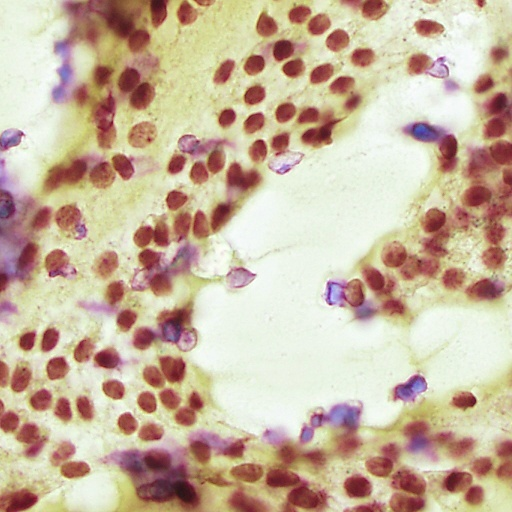
\includegraphics[width=0.48\linewidth]{figs/suggested_methods/subs/data_augmentation/jitter_1054-original.jpeg}
        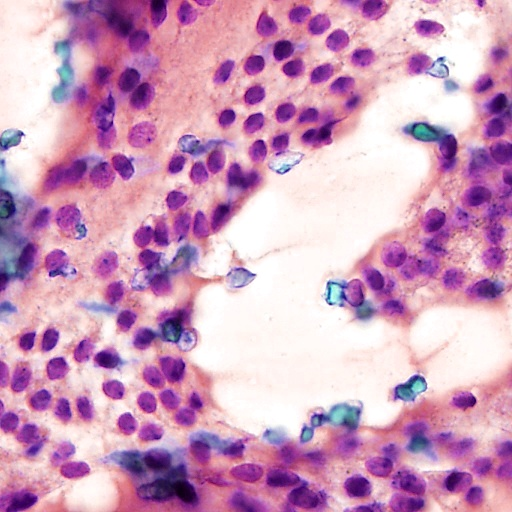
\includegraphics[width=0.48\linewidth]{figs/suggested_methods/subs/data_augmentation/jitter_1054-transformed.jpeg}
    \end{center}
    \caption{نمونه ای از پیش پردازش تغییر رنگ که به ترتیب از راست به چپ عکس اصلی و عکس تبدیل شده را نشان می دهد.}
    \label{شکل: jitter augmentation}
\end{figure}

\subsubsection{تطبیق دامنه فوریه\LTRfootnote{Fourier domain adaptation}}
%https://towardsdatascience.com/deep-domain-adaptation-in-computer-vision-8da398d3167f
در یک تنظیمات طبقه بندی، شما اغلب از یکی از معماری های شبکه استاندارد (ResNet، VGG و غیره) استفاده می کنید و آن را با استفاده از مجموعه داده خود آموزش می دهید.
این احتمالاً منجر به عملکرد بسیار خوب خواهد شد.
از سوی دیگر، اگر مجموعه داده‌هی بزرگی برای مشکل خاص خود در اختیار ندارید، CNN‌ها\LTRfootnote{Convolutional Neural Network} همچنین اجازه می‌دهند از CNNها که قبلاً شبکه‌ای را برای مشکلی مشابه آموزش داده‌اند، با انتقال یادگیری\LTRfootnote{Transfer Learning} استفاده کنید.
در این مورد، شبکه ای را انتخاب می کنید که روی یک مجموعه داده بزرگ از قبل آموزش داده شده است و برخی از لایه های بالایی آن را با استفاده از مجموعه داده های برچسب دار کوچک خود تنظیم دقیق\LTRfootnote{Fine Tune} می کنید.
هر دوی این رویکردها فرض می‌کنند که داده‌های آموزشی شما (چه بزرگ یا کوچک) نماینده خوبی از توزیع کلی داده هاست.
با این حال، اگر ورودی ها در زمان آزمون به طور قابل توجهی با داده های آموزشی متفاوت باشد، مدل ممکن است عملکرد چندان خوبی نداشته باشد.

این روش ابتدا در \cite{testi} معرفی شد.
\begin{figure}
    \begin{center}
        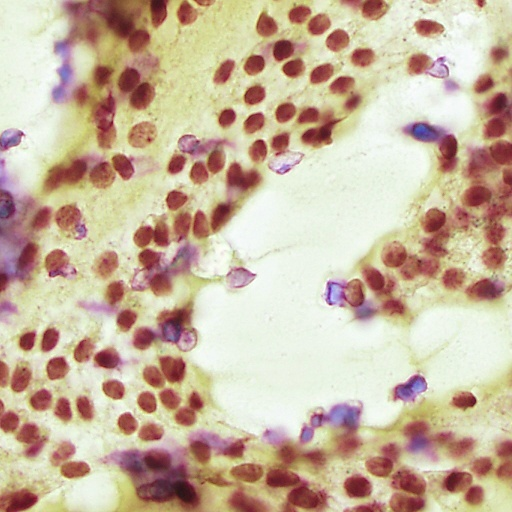
\includegraphics[width=0.48\linewidth]{figs/suggested_methods/subs/data_augmentation/fda_1054-original.jpeg}
        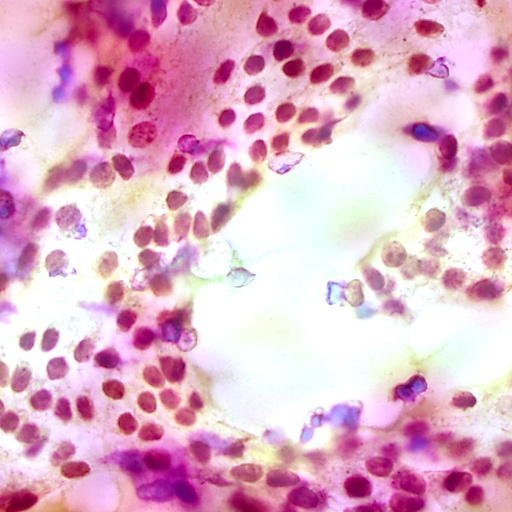
\includegraphics[width=0.48\linewidth]{figs/suggested_methods/subs/data_augmentation/fda_1054-transformed.jpeg}
    \end{center}
    \caption{نمونه ای از پیش پردازش تطبیق دامنه فوریه که به ترتیب از راست به چپ عکس اصلی و عکس تبدیل شده را نشان می دهد.}
    \label{شکل: fda augmentation}
\end{figure}

\subsubsection{ادغام تصاویر\LTRfootnote{Mix-up}}
\begin{figure}
    \begin{center}
        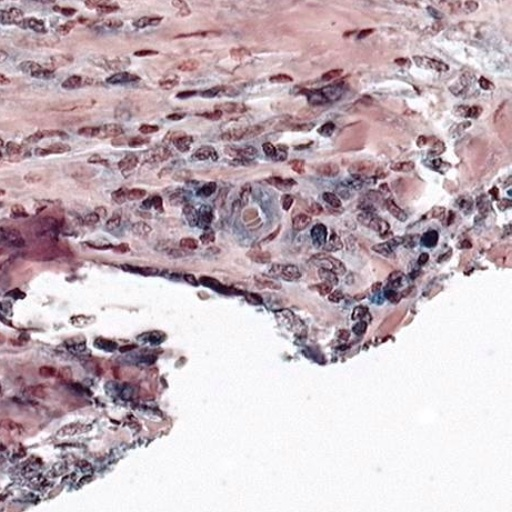
\includegraphics[width=0.48\linewidth]{figs/suggested_methods/subs/data_augmentation/mixup_776-original.jpeg}
        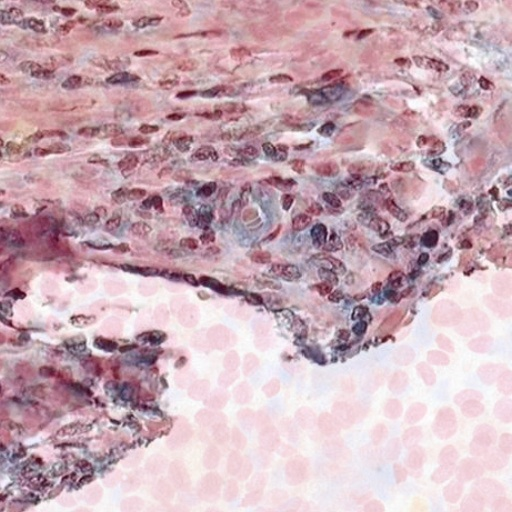
\includegraphics[width=0.48\linewidth]{figs/suggested_methods/subs/data_augmentation/mixup_776-transformed.jpeg}
    \end{center}
    \caption{نمونه ای از پیش پردازش ادغام تصویر که به ترتیب از راست به چپ عکس اصلی و عکس تبدیل شده را نشان می دهد.}
    \label{شکل: mixup augmentation}
\end{figure}
